\chapter{Ondas en cuerdas y barras: la ecuación de d'Alembert}\label{ch:b2:waves-on-strings}

Púlsese una cuerda de guitarra y una forma corre por ella, rebota en el
puente, vuelve y se asienta en el patrón estacionario cuya frecuencia se
oye como una nota. Apóyese el oído en un carril de tren y se oye el tren
mucho antes de que llegue: una compresión recorre el acero a cinco
kilómetros por segundo. El volumen del Año 1 describió esas ondas ---
progresivas, estacionarias, superpuestas --- sin decir por qué existen.
Este capítulo deduce la ecuación que las gobierna, la \emph{\omterm{thm:b2:waves-on-strings:equation}{ecuación de
ondas} de d'Alembert}, primero para el movimiento transversal de una cuerda
y después para el movimiento longitudinal de una barra construida, átomo a
átomo, con masas y resortes; calcula la energía que transporta una onda y
la impedancia que decide qué ocurre cuando encuentra un cambio de medio.

\section{La cuerda vibrante}

\begin{theorem}[Ecuación de ondas de una cuerda]\label{thm:b2:waves-on-strings:equation}
\index{ecuación de d'Alembert}\index{ecuación de ondas}\index{celeridad de las ondas (cuerda)}
Una cuerda de densidad lineal de masa $\mu$, tensada con la tensión $T$,
realiza desplazamientos transversales pequeños $y(x, t)$ (pendientes $|\partial_xy| \ll 1$). Entonces
\[
\frac{\partial^2y}{\partial t^2} = c^2\,\frac{\partial^2y}{\partial x^2} ,
\qquad c = \sqrt{\frac{T}{\mu}} ,
\]
la \emph{\omterm{thm:b2:waves-on-strings:equation}{ecuación de d'Alembert}}, cuya solución general es $y = f(x - ct)
+ g(x + ct)$: la superposición de una forma que viaja hacia la derecha y
otra que viaja hacia la izquierda a la celeridad $c$, sin deformarse.
\end{theorem}

\begin{proof}
Aíslese el elemento comprendido entre $x$ y $x + \dd x$, de masa $\mu\,\dd x$. Sus
vecinos tiran de él según la tangente a la cuerda con la tensión $T$:
horizontalmente $T\cos\theta \approx T$ en ambos extremos (no hay movimiento horizontal, así que
$T$ es la misma en toda la cuerda) y verticalmente $T\sin\theta \approx T\partial_xy$, lo que
da la fuerza neta $T[\partial_xy(x + \dd x) - \partial_xy(x)] = T\,\partial_x^2y\,\dd x$.
Newton: $\mu\,\dd x\,\partial_t^2y = T\partial_x^2y\,\dd x$. Para la solución, póngase
$u = x - ct$, $v = x + ct$: la ecuación se convierte en $\partial_u\partial_vy = 0$
(regla de la cadena), luego $\partial_vy$ depende solo de $v$ y $y = f(u) + g(v)$;
recíprocamente, toda $y$ de esa forma la satisface. Despreciar la gravedad
es legítimo cuando $T \gg \mu gL$.
\end{proof}

\begin{omfigure}
\begin{tikzpicture}[font=\small, x=1cm, y=1cm, >=Stealth]
  \begin{scope}
    \draw[->] (-2.5,0) -- (3.0,0) node[right, font=\footnotesize] {$x$};
    \draw[omDef, very thick, domain=-2.3:2.8, samples=60] plot (\x,{0.9*exp(-(\x)^2/1.6)});
    \coordinate (A) at (-0.6,{0.9*exp(-0.36/1.6)}); \coordinate (B) at (0.2,{0.9*exp(-0.04/1.6)});
    \fill[omThm] (A) circle (1.5pt); \fill[omThm] (B) circle (1.5pt);
    \draw[omThm, very thick, ->] (A) -- ($(A)+(-0.9,-0.55)$) node[above left, font=\footnotesize, yshift=2pt] {$\vect T(x)$};
    \draw[omThm, very thick, ->] (B) -- ($(B)+(1.0,-0.12)$) node[right, font=\footnotesize] {$\vect T(x+\dd x)$};
    \draw[dashed] (-0.6,0) -- (A); \draw[dashed] (0.2,0) -- (B);
    \node[font=\footnotesize] at (-0.6,-0.3) {$x$}; \node[font=\footnotesize] at (0.35,-0.3) {$x + \dd x$};
    \node[font=\footnotesize] at (0.2,-0.9) {$\mu\,\dd x\,\partial_t^2y = T\,\partial_x^2y\,\dd x$};
  \end{scope}
  \begin{scope}[xshift=7.6cm]
    \draw[->] (-2.5,0) -- (3.0,0) node[right, font=\footnotesize] {$x$};
    \draw[omDef, thick, domain=-2.3:2.8, samples=60] plot (\x,{0.8*exp(-(\x+1.3)^2/0.5)});
    \draw[omDef, thick, dashed, domain=-2.3:2.8, samples=60] plot (\x,{0.8*exp(-(\x-0.5)^2/0.5)});
    \draw[omDef, thick, ->] (-1.0,1.0) -- (0.2,1.0) node[above, font=\footnotesize, pos=0.5] {$c$};
    \node[font=\footnotesize] at (-1.3,-0.35) {$t$}; \node[font=\footnotesize] at (0.5,-0.35) {$t + \tau$};
    \node[font=\footnotesize] at (0.2,-0.9) {$y = f(x - ct)$};
  \end{scope}
\end{tikzpicture}

{\small A la izquierda, las fuerzas sobre un elemento de cuerda: las dos
tensiones no son paralelas cuando la cuerda está curvada, y su resultante
es transversal. A la derecha, una forma $f(x - ct)$ viaja hacia la derecha
a $c$ sin deformarse.}
\end{omfigure}

\begin{example}[Guitarra, piano, cable]\label{ex:b2:waves-on-strings:numbers}
La cuerda mi grave de una guitarra ($\mu = \qty{5.5}{g/m}$, longitud \qty{0.65}{m},
\qty{82.4}{Hz}) vibra en su fundamental con $\lambda = 2L$: $c = 2Lf =
\qty{107}{m/s}$ y $T = \mu c^2 = \qty{63}{N}$. La cuerda la$_4$ de un piano (acero,
\qty{1}{mm}, $\mu = \qty{6.1}{g/m}$, \qty{0.38}{m}, \qty{440}{Hz}): $c = \qty{334}{m/s}$,
$T = \qty{680}{N}$ --- y un piano tiene unas $230$ cuerdas, veinte
toneladas de tensión sobre un bastidor de fundición. Un cable de \qty{1}{kg/m} a \qty{10}{kN}:
\qty{100}{m/s}.
\end{example}

\section{Ondas estacionarias y modos}

\begin{proposition}[Modos de una cuerda fija por ambos extremos]\label{prop:b2:waves-on-strings:modes}
\index{modos propios}\index{armónicos}\index{onda estacionaria}
Una cuerda fija en $x = 0$ y en $x = L$ admite las soluciones sinusoidales
de \omterm{prop:b2:waves-on-strings:modes}{onda estacionaria} (\emph{\omterm{prop:b2:waves-on-strings:modes}{modos propios}})
\[
y_n(x, t) = A_n\sin\frac{n\pi x}{L}\cos(\omega_nt - \varphi_n) , \qquad
f_n = \frac{\omega_n}{2\pi} = n\,\frac{c}{2L} = n f_1 , \quad n = 1, 2, 3, \dots
\]
--- el fundamental $f_1 = c/2L$ y sus \emph{armónicos}. El modo $n$ tiene
$n - 1$ nodos entre los extremos. Todo movimiento de la cuerda es una
superposición $y = \sum_ny_n$, con amplitudes y fases fijadas por la forma
y la velocidad iniciales (una serie de Fourier, como establece el volumen
de matemáticas de este año): la mezcla de armónicos es el \emph{timbre} de
la nota.
\end{proposition}

\begin{proof}
Búsquese $y = F(x)\cos(\omega t - \varphi)$: $F'' + (\omega/c)^2F = 0$, $F(0) = 0$ da
$F = A\sin(\omega x/c)$, y $F(L) = 0$ exige $\omega L/c = n\pi$. Cada modo es
también la suma de dos ondas progresivas: $\sin kx\cos\omega t = \tfrac12[\sin(kx -
\omega t) + \sin(kx + \omega t)]$ --- la onda y su reflejada. La
completitud de los senos es el teorema de Fourier.
\end{proof}

\begin{omfigure}
\begin{tikzpicture}
\begin{axis}[omaxis, axis x line=bottom, axis y line=none, width=6.4cm, height=5.2cm,
    xmin=0, xmax=1, ymin=-5.9, ymax=1.5, xtick={0,1}, xticklabels={$0$, $L$}, samples=80,
    xlabel={}, ylabel={}]
  \addplot[omDef, thick, domain=0:1] {sin(deg(pi*x))};
  \addplot[omDef, thick, dashed, domain=0:1] {-sin(deg(pi*x))};
  \addplot[omThm, thick, domain=0:1] {0.8*sin(deg(2*pi*x))-2.6};
  \addplot[omThm, thick, dashed, domain=0:1] {-0.8*sin(deg(2*pi*x))-2.6};
  \addplot[omProp, thick, domain=0:1] {0.7*sin(deg(3*pi*x))-5.0};
  \addplot[omProp, thick, dashed, domain=0:1] {-0.7*sin(deg(3*pi*x))-5.0};
  \addplot[black, thin] coordinates {(0,-2.6) (1,-2.6)};
  \addplot[black, thin] coordinates {(0,-5.0) (1,-5.0)};
  \node[font=\scriptsize] at (axis cs:0.5,1.25) {$n = 1$};
  \node[font=\scriptsize] at (axis cs:0.5,-1.4) {$n = 2$};
  \node[font=\scriptsize] at (axis cs:0.5,-3.85) {$n = 3$};
\end{axis}
\end{tikzpicture}
\hfill
\begin{tikzpicture}
\begin{axis}[omaxis, axis x line=bottom, axis y line=left, width=5.0cm, height=4.2cm,
    xlabel={$x/L$}, ylabel={$y$}, xmin=0, xmax=1, ymin=-0.05, ymax=1.1, xtick={0,0.5,1}, ytick=\empty, samples=200, clip=false,
    xlabel style={at={(axis description cs:0.5,-0.12)}, anchor=north},
    ylabel style={at={(axis description cs:-0.06,0.5)}, rotate=90, anchor=south}]
  \addplot[black, thick] coordinates {(0,0) (0.5,1) (1,0)};
  \addplot[omDef, thick, domain=0:1] {0.81*sin(deg(pi*x))};
  \addplot[omThm, thick, domain=0:1] {0.81*sin(deg(pi*x)) - 0.09*sin(deg(3*pi*x))};
  \node[font=\scriptsize, anchor=west] at (axis cs:0.03,0.95) {pulsada};
  \node[font=\scriptsize, omDef, anchor=east] at (axis cs:0.97,0.95) {$n = 1$};
  \node[font=\scriptsize, omThm, anchor=east] at (axis cs:0.97,0.78) {$n = 1, 3$};
\end{axis}
\end{tikzpicture}

{\small A la izquierda, los tres primeros modos de una cuerda fija por sus
dos extremos ($f_n = nc/2L$). A la derecha, una cuerda pulsada por su punto
medio (triángulo) y los primeros términos de su serie de Fourier: solo
aparecen los armónicos impares, con amplitudes que decrecen como $1/n^2$.}
\end{omfigure}

\begin{example}[El experimento de Melde]\label{ex:b2:waves-on-strings:melde}
\index{experimento de Melde}
Una cuerda excitada por un extremo mediante un vibrador de frecuencia $f$,
con el otro extremo pasando por una polea y sosteniendo una masa $m$ (de
modo que $T = mg$): aparece una gran \omterm{prop:b2:waves-on-strings:modes}{onda estacionaria} siempre que $f$
iguala a alguna de las $f_n = (n/2L)
\sqrt{mg/\mu}$ --- resonancia del modo $n$. Para $L = \qty{1.2}{m}$, $\mu =
\qty{1.0}{g/m}$ y $f = \qty{50}{Hz}$, las masas que dan $n = 1, 2, 3$ husos
son $m_n = 4L^2f^2\mu/n^2g = 1.47/n^2$ kg: \qty{1.47}{kg}, \qty{367}{g}, \qty{163}{g}.
Pisar una cuerda de guitarra en el traste doce reduce $L$ a la mitad y
duplica $f_1$: la octava; rozarla suavemente en el punto medio sin pisarla
mata los modos impares y deja el segundo armónico --- el armónico natural.
\end{example}

\section{Energía, potencia e impedancia}

\begin{proposition}[Energía de una onda en una cuerda]\label{prop:b2:waves-on-strings:energy}
\index{densidad de energía (cuerda)}\index{flujo de energía (cuerda)}\index{impedancia (cuerda)}
Una cuerda transporta la energía por unidad de longitud y la potencia
(flujo de energía hacia $+x$)
\[
e = \tfrac12\mu\Bigl(\frac{\partial y}{\partial t}\Bigr)^2 + \tfrac12T\Bigl(\frac{\partial y}{\partial x}\Bigr)^2 ,
\qquad
\mathcal P = -T\,\frac{\partial y}{\partial x}\,\frac{\partial y}{\partial t} ,
\]
que obedecen el balance local $\partial_te + \partial_x\mathcal P = 0$. Para una
onda progresiva $y = f(x - ct)$, las densidades cinética y potencial son
iguales y $\mathcal P = Z\,(\partial_ty)^2$ con
\[
Z = \sqrt{T\mu} = \mu c = \frac Tc ,
\]
la \emph{impedancia} de la cuerda (\unit{kg/s}): el cociente entre la
fuerza transversal $-T\partial_xy$ que la cuerda ejerce sobre lo que tiene
delante y la velocidad transversal $\partial_ty$. Una onda sinusoidal de
amplitud $A$ transporta la potencia media $\langle\mathcal P\rangle = \tfrac12Z\omega^2A^2$.
\end{proposition}

\begin{proof}
El término potencial es el trabajo de la tensión al estirar el elemento:
su longitud vale
\[
\dd x\sqrt{1 + (\partial_xy)^2} \approx \dd x\bigl(1 + \tfrac12(\partial_xy)^2\bigr) ,
\]
de modo que el exceso de longitud por $T$ da $\tfrac12T(\partial_xy)^2\dd x$. La
potencia transmitida a través de $x$ hacia $+x$ es la fuerza transversal
que la parte izquierda ejerce sobre la derecha, $-T\partial_xy$, por la velocidad
$\partial_ty$. Balance:
\[
\partial_te = \mu\,\partial_ty\,\partial_t^2y + T\,\partial_xy\,\partial_x\partial_ty ,
\qquad
-\partial_x\mathcal P = T\,\partial_x^2y\,\partial_ty + T\,\partial_xy\,\partial_x\partial_ty ,
\]
iguales en virtud de la \omterm{thm:b2:waves-on-strings:equation}{ecuación de ondas}. Para $f(x - ct)$: $\partial_xy = -\partial_ty/c$, luego $\mathcal P = (T/c)
(\partial_ty)^2$ y ambas densidades valen $\tfrac12\mu(\partial_ty)^2$.
\end{proof}

\begin{proposition}[Reflexión y transmisión en una unión]\label{prop:b2:waves-on-strings:junction}
\index{coeficiente de reflexión (cuerda)}\index{coeficiente de transmisión (cuerda)}
Una onda de amplitud $A_i$ llega desde una cuerda de impedancia $Z_1$ a
otra de impedancia $Z_2$, unidas en $x = 0$. La continuidad del
desplazamiento y de la fuerza transversal en la unión da los coeficientes
en amplitud
\[
r = \frac{A_r}{A_i} = \frac{Z_1 - Z_2}{Z_1 + Z_2} , \qquad
t = \frac{A_t}{A_i} = \frac{2Z_1}{Z_1 + Z_2} ,
\]
y las fracciones de energía $R = r^2$, $\mathcal T = 4Z_1Z_2/(Z_1 + Z_2)^2$, con
$R + \mathcal T = 1$. Un extremo fijo ($Z_2 \to \infty$) refleja con $r = -1$
(el pulso vuelve invertido); uno libre ($Z_2 = 0$), con $r = +1$;
impedancias iguales lo transmiten todo.
\end{proposition}

\begin{proof}
Ondas sinusoidales $y_1 = A_i\cos(\omega t - k_1x) + A_r\cos(\omega t + k_1x)$ para
$x < 0$ e $y_2 = A_t\cos(\omega t - k_2x)$ para $x > 0$, con la misma $\omega$ a ambos
lados. En $x = 0$: $y_1 = y_2$ da $A_i + A_r = A_t$; la continuidad de la fuerza $-T\partial_xy$
(unión sin masa) da $Z_1(A_i - A_r) = Z_2A_t$ (usando
$T_1k_1 = Z_1\omega$). Resuélvase. Energías: las potencias medias $\tfrac12Z\omega^2A^2$.
\end{proof}

\begin{omfigure}
\begin{tikzpicture}[font=\small, x=1cm, y=1cm, >=Stealth]
  \begin{scope}
    \draw[->] (-3.2,0) -- (3.2,0) node[right, font=\footnotesize] {$x$};
    \draw[omDef, very thick, domain=-3.0:0, samples=50] plot (\x,{0.8*exp(-(\x+1.6)^2/0.25)});
    \draw[omDef, very thick, domain=0:3.0, samples=50] plot (\x,{0});
    \fill (0,0) circle (2pt); \node[font=\footnotesize] at (0,-0.35) {$Z_1 \to Z_2$};
    \draw[omDef, ->, thick] (-1.6,1.0) -- (-0.8,1.0) node[above, font=\footnotesize, pos=0.5] {$A_i$};
    \node[font=\footnotesize] at (-1.5,-0.6) {$Z_1$}; \node[font=\footnotesize] at (1.5,-0.6) {$Z_2 > Z_1$};
    \node[font=\footnotesize] at (0,-1.1) {antes};
  \end{scope}
  \begin{scope}[xshift=7.2cm]
    \draw[->] (-3.2,0) -- (3.2,0) node[right, font=\footnotesize] {$x$};
    \draw[omThm, very thick, domain=-3.0:0, samples=50] plot (\x,{-0.27*exp(-(\x+1.6)^2/0.25)});
    \draw[omProp, very thick, domain=0:3.0, samples=50] plot (\x,{0.53*exp(-(\x-1.1)^2/0.12)});
    \fill (0,0) circle (2pt);
    \draw[omThm, ->, thick] (-1.0,0.5) -- (-1.8,0.5) node[above, font=\footnotesize, pos=0.5] {$rA_i$};
    \draw[omProp, ->, thick] (1.0,0.9) -- (1.8,0.9) node[above, font=\footnotesize, pos=0.5] {$tA_i$};
    \node[font=\footnotesize] at (0,-1.1) {después: $r = \dfrac{Z_1 - Z_2}{Z_1 + Z_2}$, $t = \dfrac{2Z_1}{Z_1 + Z_2}$};
  \end{scope}
\end{tikzpicture}

{\small Un pulso encuentra una unión con una cuerda más pesada ($Z_2 = 4Z_1$):
una parte se transmite, más lenta y más estrecha, y otra se refleja invertida.}
\end{omfigure}

\section{De la cadena de átomos a la barra elástica}

\begin{proposition}[La cadena de átomos; el módulo de Young]\label{prop:b2:waves-on-strings:chain}
\index{cadena de átomos}\index{módulo de Young}\index{ley de Hooke}\index{onda longitudinal}
Una fila de masas idénticas $m$ separadas por $a$ y unidas por resortes de
constante $k$: si $u_n(t)$ es el desplazamiento de la masa $n$ a lo largo
de la fila,
\[
m\ddot u_n = k(u_{n+1} - u_n) - k(u_n - u_{n-1}) = k(u_{n+1} - 2u_n + u_{n-1}) .
\]
Cuando el desplazamiento varía despacio de una masa a la siguiente (para
longitudes de onda $\lambda \gg a$), $u_n(t) \to u(x, t)$ con $u_{n\pm1} - u_n \approx
\pm a\,\partial_xu + \tfrac12a^2\partial_x^2u$, y la cadena obedece la \omterm{thm:b2:waves-on-strings:equation}{ecuación de
d'Alembert}
\[
\frac{\partial^2u}{\partial t^2} = c^2\frac{\partial^2u}{\partial x^2} , \qquad
c = a\sqrt{\frac km} = \sqrt{\frac{E}{\rho}} ,
\]
con $\rho = m/a^3$ la densidad de un sólido formado por tales cadenas en
una red cúbica y $E = k/a$ su \emph{\omterm{prop:b2:waves-on-strings:chain}{módulo de Young}}: la rigidez de una
barra de sección $S$ y longitud $\ell$ vale $kS/a^2\cdot a/\ell = ES/\ell$,
es decir, la \emph{\omterm{prop:b2:waves-on-strings:chain}{ley de Hooke}} $F/S = E\,\Delta\ell/\ell$ (esfuerzo $\sigma = E\varepsilon$).
\end{proposition}

\begin{proof}
Cada resorte se estira en la diferencia de los desplazamientos de sus
extremos. Insértense los desarrollos de Taylor: $m\partial_t^2u = ka^2\partial_x^2u$. Un cubo de
lado $a$ por átomo da $\rho = m/a^3$; una barra de sección $S$ contiene
$S/a^2$ cadenas paralelas de $\ell/a$ resortes en serie, de rigidez total
$(S/a^2)(ka/\ell) = (k/a)S/\ell$.
\end{proof}

\begin{proposition}[Ondas longitudinales en una barra]\label{prop:b2:waves-on-strings:rod}
\index{sonido en los sólidos}
Directamente sobre el medio continuo: un elemento de barra entre $x$ y $x +
\dd x$, desplazado en $u(x, t)$, se deforma en $\varepsilon = \partial_xu$ y sus
dos caras lo tiran con el esfuerzo $\sigma = E\partial_xu$; Newton da $\rho\,\partial_t^2u =
E\,\partial_x^2u$: las \omterm{prop:b2:waves-on-strings:chain}{ondas longitudinales} (de compresión) viajan a $c = \sqrt{E/\rho}$
--- \qty{5100}{m/s} en el acero ($E = \qty{200}{GPa}$), \qty{5000}{m/s} en el aluminio,
\qty{3700}{m/s} en el granito, \qty{3500}{m/s} en la madera según la fibra. La
impedancia vale $Z = \rho c = \sqrt{E\rho}$ por unidad de área, y valen las
mismas fórmulas de unión --- así es como los ultrasonidos encuentran una
grieta en un carril.
\end{proposition}

\begin{proof}
Fuerza neta sobre el elemento: $S[\sigma(x + \dd x) - \sigma(x)] = SE\partial_x^2u\,\dd x$;
masa $\rho S\dd x$.
\end{proof}

\begin{omfigure}
\begin{tikzpicture}[font=\small, x=1cm, y=1cm, >=Stealth]
  \begin{scope}
    \foreach \i in {0,1,2,3,4} {
      \fill[omDef] ({1.4*\i},0) circle (5pt);
    }
    \foreach \i in {0,1,2,3} {
      \draw[thick, decorate, decoration={coil, aspect=0.5, segment length=4pt, amplitude=3pt}] ({1.4*\i+0.18},0) -- ({1.4*\i+1.22},0);
    }
    \node[font=\footnotesize] at (1.4,-0.5) {$u_{n-1}$}; \node[font=\footnotesize] at (2.8,-0.5) {$u_n$}; \node[font=\footnotesize] at (4.2,-0.5) {$u_{n+1}$};
    \draw[<->] (1.4,0.45) -- (2.8,0.45) node[midway, above, font=\footnotesize] {$a$};
    \node[font=\footnotesize] at (2.8,-1.1) {$m\ddot u_n = k(u_{n+1} - 2u_n + u_{n-1})$};
  \end{scope}
  \begin{scope}[xshift=8.0cm]
    \draw[thick] (-2.0,-0.5) rectangle (2.6,0.5);
    \fill[omDef!25] (-0.3,-0.5) rectangle (0.5,0.5);
    \draw[omThm, very thick, ->] (-0.3,0) -- (-1.2,0) node[above, font=\footnotesize, pos=0.6] {$\sigma(x)S$};
    \draw[omThm, very thick, ->] (0.5,0) -- (1.5,0) node[above, font=\footnotesize, pos=0.6] {$\sigma(x + \dd x)S$};
    \node[font=\footnotesize] at (0.1,-0.8) {$\rho S\dd x\,\partial_t^2u = SE\,\partial_x^2u\,\dd x$};
    \node[font=\footnotesize] at (0.3,-1.35) {$c = \sqrt{E/\rho}$};
  \end{scope}
\end{tikzpicture}

{\small A la izquierda, la cadena de masas y resortes: cada masa siente
los dos resortes que la rodean, y el límite continuo es la \omterm{thm:b2:waves-on-strings:equation}{ecuación de ondas}
con $c = a\sqrt{k/m}$. A la derecha, un elemento de barra elástica tirado
por el esfuerzo sobre sus dos caras.}
\end{omfigure}

\begin{remark}[Lo que la cadena sabe y la barra no]\label{rem:b2:waves-on-strings:dispersion}
Buscar $u_n = A\cos(\omega t - kna)$ en la ecuación exacta de la cadena da
$\omega = 2\sqrt{k/m}\,|\sin(ka/2)|$: para $ka \ll 1$ esto es $\omega = ck$, la
\omterm{thm:b2:waves-on-strings:equation}{ecuación de ondas} no dispersiva, pero a medida que la longitud de onda se acerca a $2a$ la
frecuencia se satura en $2\sqrt{k/m}$ y las velocidades de fase y de grupo
difieren --- la primera \emph{relación de dispersión} de este volumen,
tema de \cref{ch:b2:dispersion-wave-packets}. Para $a = \qty{0.25}{nm}$ y
$c = \qty{5}{km/s}$ el corte está en $\omega_{\max} = 2c/a = \qty{4e13}{rad/s}$
(\qty{6}{THz}): el sólido no puede vibrar más deprisa de lo que permiten
los resortes de sus átomos.
\end{remark}

\section{Ejercicios}

\begin{exercise}[$\star$]\label{exo:b2:waves-on-strings:1}
La cuerda la de una guitarra (\qty{110}{Hz}, $L = \qty{65}{cm}$, $\mu = \qty{3.0}{g/m}$):
celeridad de las ondas, tensión, longitud de onda del fundamental en la
cuerda y del sonido en el aire; frecuencia al pisar la cuerda en el quinto
traste ($L$ reducida en un factor $2^{-5/12}$).
\end{exercise}

\begin{exercise}[$\star$]\label{exo:b2:waves-on-strings:2}
Celeridad de las \omterm{prop:b2:waves-on-strings:chain}{ondas longitudinales} en el acero ($E = \qty{200}{GPa}$, $\rho =
\qty{7800}{kg/m^3}$), el aluminio (\qty{70}{GPa}, \qty{2700}{kg/m^3}) y el plomo
(\qty{16}{GPa}, \qty{11300}{kg/m^3}). Tiempo que tarda un sonido en recorrer \qty{1.0}{km}
por un carril y por el aire (\qty{340}{m/s}); qué oye quien tiene el oído
apoyado en el carril.
\end{exercise}

\begin{exercise}[$\star$]\label{exo:b2:waves-on-strings:3}
Una cuerda de fundamental \qty{200}{Hz}: frecuencias y número de nodos de
los modos 2, 3 y 4; posiciones de los nodos del modo 3; frecuencia del
fundamental si se duplica la tensión, si se reduce la longitud a la mitad
y si se sustituye la cuerda por otra tres veces más pesada por metro.
\end{exercise}

\begin{exercise}[$\star$]\label{exo:b2:waves-on-strings:4}
Una cuerda de \qty{12}{m} ($\mu = \qty{0.20}{kg/m}$) se tensa con \qty{45}{N};
un extremo está fijo a una pared. Se lanza un pulso desde el otro extremo.
Celeridad; tiempo en llegar a la pared y volver; forma del pulso que
vuelve; lo mismo si el extremo lejano está atado a una anilla ligera que
desliza libremente por un poste.
\end{exercise}

\begin{exercise}[$\star\star$]\label{exo:b2:waves-on-strings:5}
Una cuerda de piano para \qty{440}{Hz}: acero ($\rho = \qty{7800}{kg/m^3}$),
diámetro \qty{1.0}{mm}, longitud vibrante \qty{38}{cm}. (a) $\mu$, celeridad
de las ondas y tensión. (b) Esfuerzo en el alambre; compárese con la
resistencia del alambre de piano, unos \qty{2}{GPa}. (c) La misma nota con un alambre de \qty{0.5}{mm}: tensión
y esfuerzo. (d) ¿Por qué se entorchan con cobre las cuerdas graves en vez
de hacerlas más largas o más gruesas?
\end{exercise}

\begin{exercise}[$\star\star$]\label{exo:b2:waves-on-strings:6}
\emph{Melde.} Una cuerda de \qty{1.5}{m} ($\mu = \qty{2.0}{g/m}$) se excita a
\qty{60}{Hz}; su tensión la fija una masa colgada. (a) Masas que dan
$1$, $2$, $3$ y $4$ husos. (b) Con \qty{0.50}{kg}: ¿hay resonancia?
El modo más próximo. (c) ¿Es el extremo excitado un nodo o un vientre?
(d) ¿Por qué crecen tanto los husos en resonancia y qué los limita?
\end{exercise}

\begin{exercise}[$\star\star$]\label{exo:b2:waves-on-strings:7}
Una onda $y = A\cos(\omega t - kx)$ con $A = \qty{2.0}{mm}$ y $f = \qty{100}{Hz}$
viaja por una cuerda ($T = \qty{100}{N}$, $\mu = \qty{10}{g/m}$). Celeridad, $k$
y longitud de onda; velocidad y aceleración transversales máximas de un
punto; pendiente máxima; impedancia; potencia media transportada; energía
contenida en una longitud de onda.
\end{exercise}

\begin{exercise}[$\star\star$]\label{exo:b2:waves-on-strings:8}
Una cuerda de $\mu_1 = \qty{2.0}{g/m}$ está atada a otra de $\mu_2 = \qty{8.0}{g/m}$,
ambas a \qty{20}{N}. (a) Celeridades e impedancias. (b) Coeficientes de
reflexión y de transmisión en amplitud para una onda que llega desde la
cuerda ligera; y desde la pesada. (c) Fracciones de energía en ambos
casos; compruébese que suman uno. (d) Un pulso de \qty{1}{cm} de altura y \qty{10}{cm} de anchura
llega desde la cuerda ligera: altura y anchura de los pulsos transmitido y
reflejado.
\end{exercise}

\begin{exercise}[$\star\star$]\label{exo:b2:waves-on-strings:9}
Un alambre de acero de \qty{2.0}{m} y \qty{1.0}{mm} de diámetro se alarga \qty{1.0}{mm}
bajo \qty{80}{N}. (a) \omterm{prop:b2:waves-on-strings:chain}{Módulo de Young}. (b) Celeridad de las \omterm{prop:b2:waves-on-strings:chain}{ondas longitudinales}.
(c) Frecuencia fundamental de la vibración longitudinal del alambre
empotrado por ambos extremos, y de su vibración transversal con esa
tensión; ¿por qué son tan distintas? (d) Constante $k$ y masa $m$ de un
``átomo'' en el modelo de cadena, para $a = \qty{0.25}{nm}$.
\end{exercise}

\begin{exercise}[$\star\star\star$]\label{exo:b2:waves-on-strings:10}
\emph{La cuerda pulsada.} Una cuerda fija en $0$ y en $L$ se separa
lateralmente en $x = L/2$ hasta la altura $h$ (forma triangular) y se
suelta en reposo. (a) Escríbase la solución como $\sum_nb_n\sin(n\pi x/L)\cos(\omega_nt)$ y muéstrese
que $b_n = \dfrac{8h}{n^2\pi^2}\sin\dfrac{n\pi}2$. (b) ¿Qué armónicos
faltan y por qué? (c) Energía del modo $n$ ($E_n = \tfrac14\mu L\omega_n^2b_n^2$);
fracción del total que se lleva el fundamental. (d) La cuerda se pulsa en
$L/5$: ¿qué armónicos se anulan? ¿Por qué pulsa un guitarrista cerca del
puente para obtener un sonido más brillante?
\end{exercise}

\begin{exercise}[$\star\star\star$]\label{exo:b2:waves-on-strings:11}
\emph{Dispersión de la cadena.} (a) Insértese $u_n = A\cos(\omega t - kna)$ en
la ecuación de la cadena y dedúzcase $\omega(k) = 2\omega_0|\sin(ka/2)|$, $\omega_0 =
\sqrt{k/m}$. (b) Velocidad de fase $\omega/k$ y velocidad de grupo $\dd\omega/\dd k$;
su límite común para $ka \to 0$; sus valores en $ka = \pi$. (c) ¿Qué aspecto
tiene la onda en $ka = \pi$? ¿Por qué no hay ondas de longitud de onda
menor que $2a$? (d) Para el acero ($c = \qty{5.1}{km/s}$, $a =
\qty{0.25}{nm}$): $\omega_0$, la frecuencia máxima y la longitud de onda de un
ultrasonido de \qty{1}{MHz} --- ¿es dispersivo?
\end{exercise}

\begin{exercise}[$\star\star\star$]\label{exo:b2:waves-on-strings:12}
\emph{Cuerda colgante, látigo que restalla.} (a) Una cuerda homogénea de
longitud $L$ cuelga del techo: tensión a la altura $x$ sobre el extremo
libre; celeridad local de las ondas $c(x)$. (b) Tiempo que tarda un pulso
en subir de abajo arriba; valor para $L = \qty{10}{m}$; por qué cambia la
forma del pulso. (c) Un látigo se afila y su $\mu$ decrece hacia la punta,
con tensión (casi) constante durante el golpe: ¿cómo varía la celeridad a
lo largo de él? (d) Admitiendo que la energía del pulso se conserva y que
su duración se mantiene constante, muéstrese que la amplitud de su
velocidad transversal crece como $\mu^{-1/4}$, y estímese la celeridad de
la punta de un látigo cuya $\mu$ cae en un factor $10^4$ del mango a la
punta si la mano le comunica \qty{10}{m/s}. (El restallido es una explosión sónica.)
\end{exercise}

\begin{omfigure}
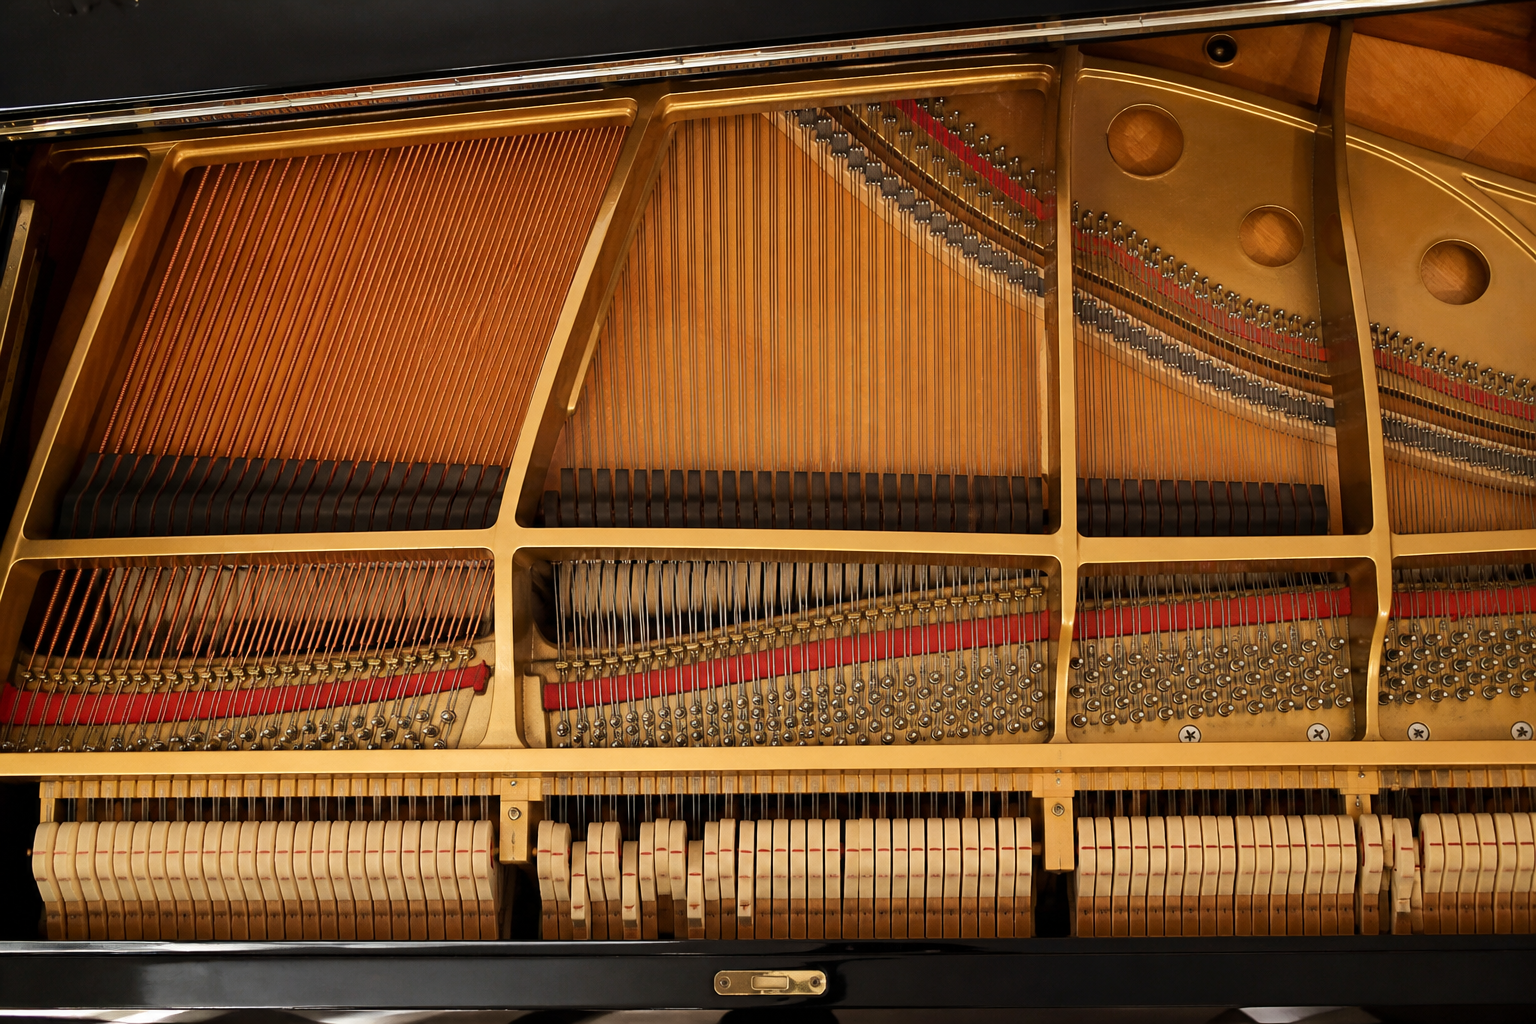
\includegraphics[width=0.58\linewidth]{images/book4/ai/b4-06-grand-piano-strings.png}

{\small El interior de un piano de cola: unas doscientas cuerdas de acero de longitud y grosor graduados, cada una afinada por su tensión a un fundamental $c/2L$; las cuerdas graves van entorchadas con cobre para ganar masa.}
\end{omfigure}

\section{Problema: el piano, del macillo a la tabla armónica}

\begin{problem}[{Problema de fin de semana --- una cuerda de piano
desmontada: su tensión y su rigidez, el golpe del macillo y los armónicos
que crea, el puente que fuga su energía hacia la tabla armónica, y un
carril que obedece la misma ecuación}]
\label{pb:b2:waves-on-strings:1}

\medskip
\noindent\textbf{Parte I --- La cuerda.}
La cuerda la$_4$ de un piano (\qty{440}{Hz}): acero, $E = \qty{200}{GPa}$, $\rho =
\qty{7800}{kg/m^3}$, diámetro $d = \qty{1.0}{mm}$, longitud vibrante $L =
\qty{38}{cm}$. Cada nota por encima de los graves tiene tres cuerdas así; el
piano tiene $230$ cuerdas.
\begin{enumerate}
  \item Densidad lineal de masa, celeridad de las ondas y tensión de la
        cuerda.
  \item Esfuerzo de tracción en el alambre; el alambre rompe a
        \qty{2.0}{GPa}: margen de seguridad y por qué la última vuelta del
        afinador es la peligrosa.
  \item Estímese la tensión total sobre el bastidor, tomando todas las
        cuerdas a la misma tensión.
  \item La cuerda más grave (la$_0$, \qty{27.5}{Hz}) mide \qty{1.9}{m}; si
        fuese un simple alambre de acero a la misma tensión, ¿qué $\mu$ y
        qué diámetro necesitaría? En realidad es un alma de acero
        entorchada con cobre: explíquese.
  \item Modos de la cuerda la$_4$: frecuencias de los ocho primeros
        armónicos; ¿cuáles caen en un intervalo consonante con el
        fundamental (octava, quinta, cuarta, tercera mayor) y cuáles no?
  \item La cuerda vibra en su fundamental con una amplitud de
        \qty{0.50}{mm} en el vientre: energía almacenada (la energía de un
        modo vale $\tfrac14\mu L\omega^2A^2$).
  \item Escríbase el fundamental como suma de dos ondas progresivas; dense
        su amplitud y la potencia media que transporta cada una.
\end{enumerate}

\medskip
\noindent\textbf{Parte II --- El macillo.}
El macillo golpea la cuerda en $x_0 = L/8$ y le comunica, en $t = 0$, una
velocidad $v_0$ sobre un segmento corto de anchura $w$ en torno a $x_0$,
sin desplazamiento.
\begin{enumerate}[resume]
  \item Escríbase la solución general $y = \sum_nB_n\sin(n\pi x/L)\sin(\omega_nt)$
        y muéstrese, usando la ortogonalidad de los senos, que $B_n =
        \dfrac{2}{L\omega_n}\int_0^L\dot y(x, 0)\sin\dfrac{n\pi x}L\,\dd x$.
  \item Para un golpe estrecho ($w \ll L/n$), muéstrese que $B_n \approx \dfrac{2v_0w}
        {L\omega_n}\sin\dfrac{n\pi x_0}{L}$.
  \item ¿Qué armónicos faltan para $x_0 = L/8$? ¿Por qué golpean los
        constructores de pianos cerca de $L/7$ o de $L/8$ (véase la pregunta 5)?
  \item Descríbase el movimiento en la imagen de ondas progresivas: qué
        sale del punto golpeado, qué ocurre en los extremos y al cabo de
        cuánto tiempo se repite el estado inicial.
  \item Una cuerda real es algo rígida: sus modos son $f_n = nf_1
        \sqrt{1 + Bn^2}$ con $B = \pi^3Ed^4/(64TL^2)$ (admitido). Calcúlense
        $B$ y la elevación del octavo armónico, en tanto por ciento y
        en cents (\qty{1}{cent} = una razón de frecuencias $2^{1/1200}$).
  \item ¿Por qué los afinadores ``estiran'' las octavas (afinan las notas
        agudas un poco altas)?
\end{enumerate}

\medskip
\noindent\textbf{Parte III --- El puente y la tabla armónica.}
La cuerda pasa por un puente encolado a la tabla armónica; la tabla se
comporta, en el puente, como una cuerda de impedancia $Z_b = \qty{2000}{kg/s}$.
\begin{enumerate}[resume]
  \item Impedancia $Z_s$ de la cuerda; coeficiente de reflexión en
        amplitud en el puente.
  \item Fracción de la energía de la onda transmitida a la tabla armónica
        en cada reflexión.
  \item Número de reflexiones por segundo en el puente; dedúzcanse la
        constante de tiempo de la caída de la energía y el tiempo que
        tarda el sonido en bajar \qty{60}{dB} (un factor $10^6$ en energía).
  \item Potencia que se fuga hacia la tabla armónica justo después del
        golpe de la pregunta 6; compárese con la potencia de una
        conversación tranquila, unos \qty{1e-5}{W} de sonido.
  \item ¿Por qué es casi inaudible una cuerda sola y qué hace la tabla
        armónica al respecto? (Piénsese en la impedancia del aire,
        $\rho c \approx \qty{400}{kg.m^{-2}.s^{-1}}$, vista a través de una
        superficie pequeña frente a una grande.)
  \item Con el apagador levantado, la cuerda la$_3$ (\qty{220}{Hz}) empieza
        a sonar cuando se toca la$_4$: ¿por qué?
  \item Un constructor quiere un sonido más prolongado: ¿debe subir o
        bajar $Z_b$, y qué se pierde?
\end{enumerate}

\medskip
\noindent\textbf{Parte IV --- El carril.}
Un carril de acero ($E = \qty{200}{GPa}$, $\rho = \qty{7800}{kg/m^3}$, sección
\qty{70}{cm^2}).
\begin{enumerate}[resume]
  \item Celeridad de las ondas de compresión; tiempo que tarda el sonido
        de un tren en recorrer \qty{5}{km} por el carril y por el aire.
  \item Un martillazo lanza un pulso de compresión por un tramo de carril
        de \qty{25}{m} con un extremo libre: tiempo del eco; ¿es el eco una
        compresión o una dilatación?
  \item Una sonda ultrasónica de \qty{2}{MHz} busca grietas: longitud de
        onda en el acero; coeficiente de reflexión en amplitud en una
        grieta acero--aire (impedancia del aire
        $\qty{400}{kg.m^{-2}.s^{-1}}$); por qué se ve tan bien una grieta
        fina.
  \item Terremotos: en la roca, las ondas de compresión (P) viajan a
        \qty{6.0}{km/s} y las de cizalla (S) a \qty{3.5}{km/s}. Una estación
        registra la onda S \qty{20}{s} después de la P: distancia al foco.
  \item Reúnanse en una tabla las cinco celeridades de onda de este
        problema (cuerda, carril, roca P, roca S, aire) con la rigidez y
        la inercia que fijan cada una.
\end{enumerate}
\end{problem}
